\chapter*{Annexe 4 - Commande à temps discret}
\addcontentsline{toc}{chapter}{Commande à temps discret}
%\setcounter{section}{0}
% **********************************

%\label{Annex:comTD}
\lstset{
  language=Matlab,                	  % choose the language of the code
  basicstyle=\ttfamily,
  numbers=left,                   % where to put the line-numbers
  stepnumber=1,                   % the step between two line-numbers.
  numbersep=5pt,                  % how far the line-numbers are from the code
  backgroundcolor=\color{white},  % choose the background color. You must add \usepackage{color}
  commentstyle = \color{darkgreen},
  showspaces=false,               % show spaces adding particular underscores
  showstringspaces=false,         % underline spaces within strings
  showtabs=false,                 % show tabs within strings adding particular underscores
  tabsize=2,                      % sets default tabsize to 2 spaces
  captionpos=b,                   % sets the caption-position to bottom
  breaklines=true,                % sets automatic line breaking
  breakatwhitespace=true,         % sets if automatic breaks should only happen at whitespace
  %caption=exo1.m,                 % show the filename of files included with \lstinputlisting;
  literate={á}{{\'a}}1 {è}{{\`e}}1 {é}{{\'e}}1,
}
\section*{Modèles $SIMULNK$}
\addcontentsline{toc}{section}{Modèles $SIMULNK$}

\begin{figure}[!ht]
	\centering
	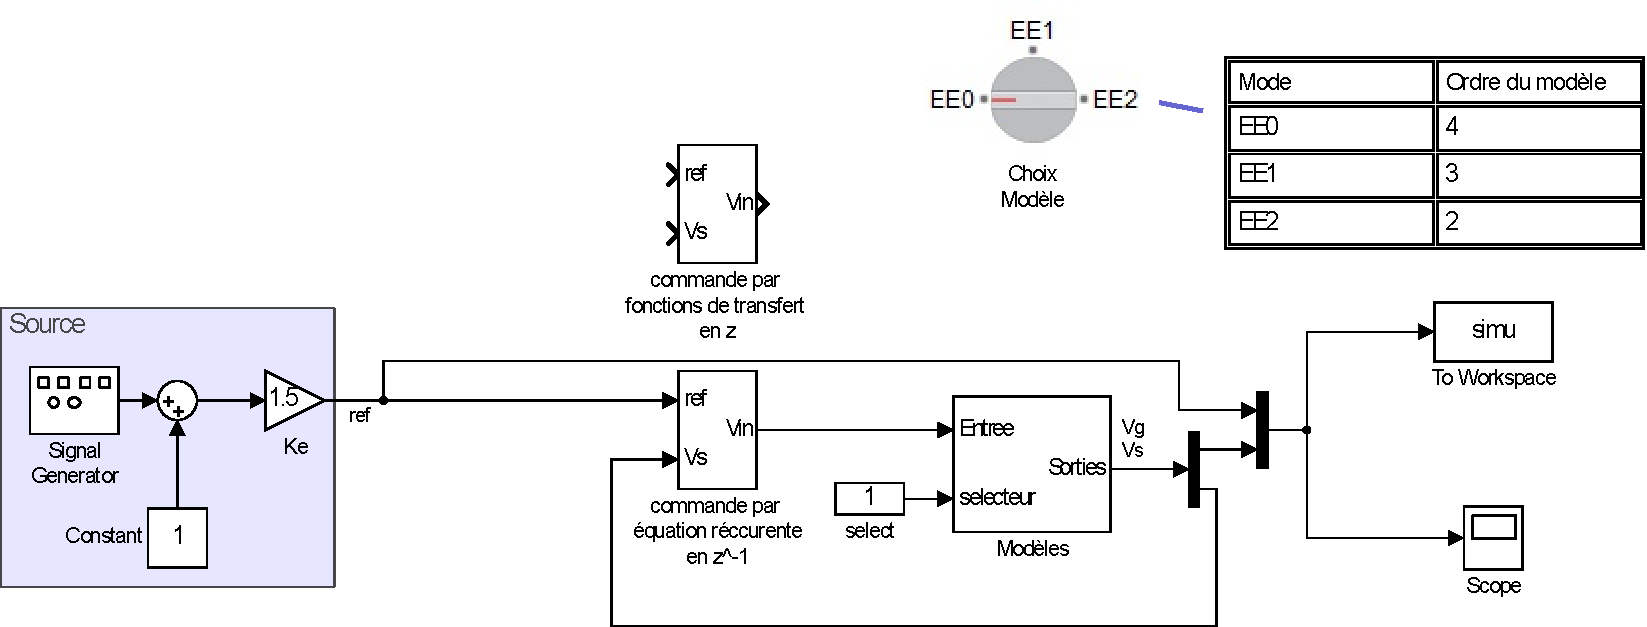
\includegraphics[width = \textwidth]{./annexes/annexe4/Commande_TD_general.pdf}
	\caption{\emph{SIMULINK :} Modèle général}
\end{figure}

\begin{figure}[!ht]
	\centering
	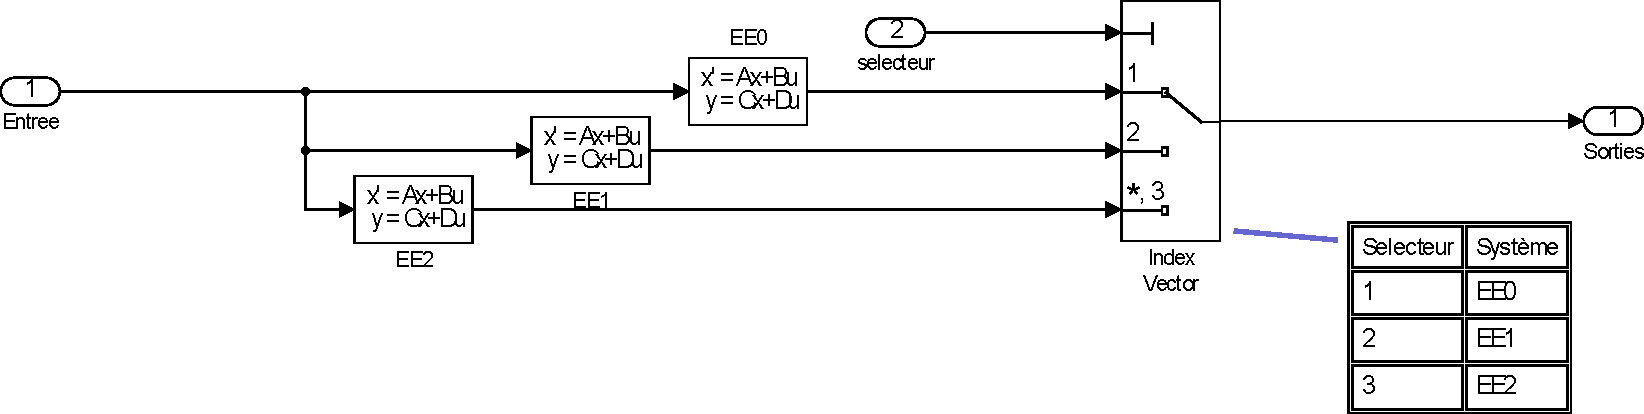
\includegraphics[width = \textwidth]{./annexes/annexe4/Commande_TD_modele.pdf}
	\caption{\emph{SIMULINK :} Subsystem des modèles}
\end{figure}

\begin{figure}[!ht]
	\centering
	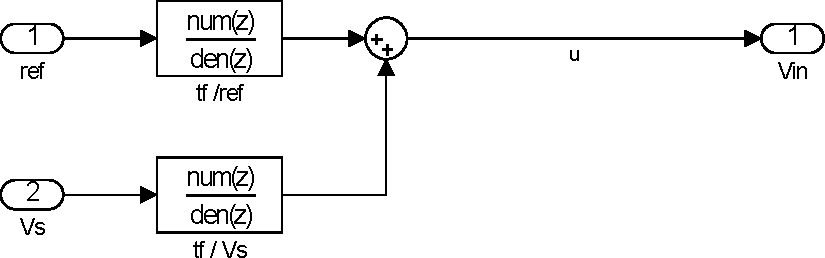
\includegraphics[width = .6\textwidth]{./annexes/annexe4/Commande_TD_comFT.pdf}
	\caption{\emph{SIMULINK :} Subsystem de la commande par fonctions de transferts}
\end{figure}

\begin{figure}[!ht]
	\centering
	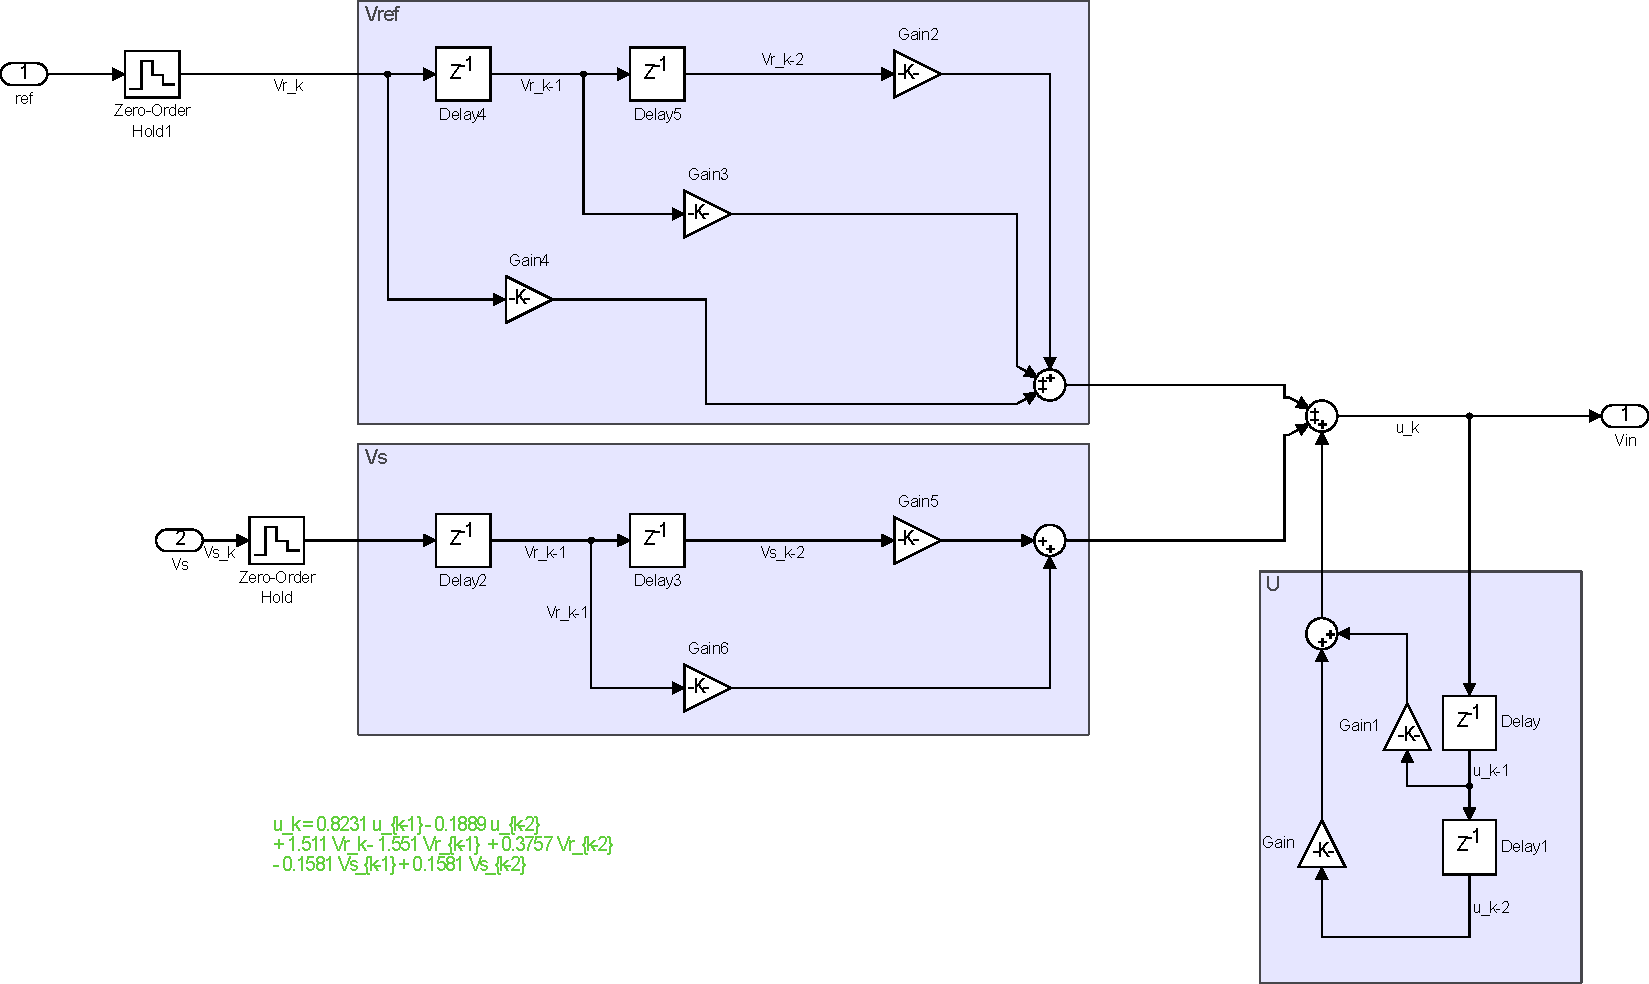
\includegraphics[width = \textwidth]{./annexes/annexe4/Commande_TD_comER.pdf}
	\caption{\emph{SIMULINK :} Subsystem de la commande par équation récurrente}
\end{figure}
\section*{Script Matlab}
\addcontentsline{toc}{section}{Modèles $SIMULNK$}
\lstset{caption=Script d'affichage}
\lstinputlisting{./annexes/annexe4/affichage.m}